\chapter{Introduzione al fenomeno della lingua}
\section{Significato e significante}

\begin{abstract}
Il linguaggio è uno strumento per trasmettere informazioni attraverso una serie di simboli. Ma cosa è un simbolo? Dato un oggetto (significato), un simbolo è ciò che lo rappresenta (significante).
I veicoli segnici rappresentano i sensi delle parole (che sono nell'iperuranio/nella testa dei parlanti).
\end{abstract}

\begin{figure}
    \centering
    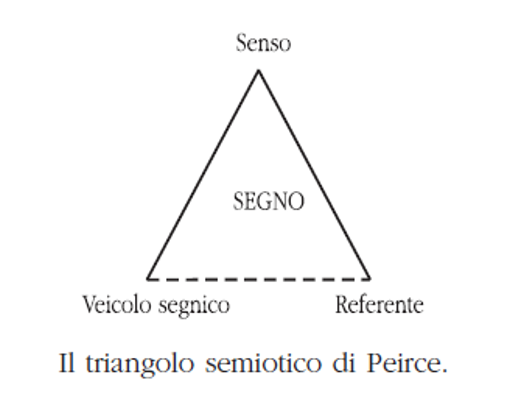
\includegraphics[width=0.5\linewidth]{peirce.PNG}
    \caption{Triangolo di Peirce}
    \label{fig:enter-label}
\end{figure}

\begin{abstract}
Tuttavi andare dal veicolo segnico al senso e viceversa non è immediato poichè la relazione è 'molti a molti', infatti, la rappresentazione naturale soffre di molti "difetti", come ad esempio la ricchezza espressiva(più veicoli segnici vanno in un unico senso), l'arbitrarietà e l'ambiguità (più sensi vanno in uno stesso veicolo segnico).
\begin{Oss}{Esempio:} Una vecchia legge la regola \end{Oss}
Esistono però vari tipi di ambiguità in base al livello linguistico in cui ci troviamo.
\end{abstract}

%%%%%%%%%%%%%%%%%%%%%%%%%%%%%%%%%%%
\section{Livelli linguistici}

\begin{abstract}
Fonologia: branca della linguistica che studia i sistemi di suoni; la più semplice particella che studia la fonologia è il \textbf{fonema}, che può essere un singolo suono.
\end{abstract}

\begin{abstract}
Morfologia: è lo studio delle parole, la loro composizione, e l'appartenenza a determinate categorie (nome, verbo, etc...).
Nella linguistica moderna studia la struttura della parola e descrive le varie forme che assume a seconda delle categorie di numero, genere, modo, tempo e persona.
Le parole sono costituite di \textbf{morfemi}, unità minime con significato autonomo, ..
\end{abstract}

\begin{abstract}
Sinstassi: branca della grammatica e linguistica che studia i diversi modi (relazioni) in cui i codici dei linguaggi si uniscono fra loro per formare una preposizione, "unità superiori alla parola". 
\end{abstract}

\begin{abstract}
Sematica: studio del significato delle parole (lessicale), e delle frasi (frasale), considerando il rapporto fra l'espressione e la realtà extralinguistica. Il significato di una frase è dato da quello delle singole parti, più quello degli eventuali elementi connettori (anche se non è detto che ciò sia sufficiente, considerando ad esempio metafore o catacresi).
\end{abstract}

\begin{abstract}
Pragmatica: studio del linguaggio in rapporto all'uso contestuale che ne fa il parlante, come il contesto contribuisce al significato.
\end{abstract}

%%%%%%%%%%%%%%%%%%%%%%%%%%%%%%%%%%%
\section{Interpreting Natural Language}

\begin{abstract}
Abbiamo stabilito che lo scopo de linguggio naturale è la comunicazione, trasmettere idee sul mondo interiore o esteriore, credenze, knowledge, concetti, emozioni... ma come lo interpretiamo?
Dati dei concetti e le relazioni fra essi vogliamo ricavare istanze, fatti accaduti. -> Retriving information from text collection
Vogliamo definire un meccanismo (finito) che possa generare ed interpretare un linguaggio:
    \begin{itemize}
        \item interpretare: da una frase costruire il grafo(albero) di derivazione;
        \item generare: dal grafo ricostruire la frase;
    \end{itemize}
\end{abstract}

\section{Classi sintattiche e costituenti}
\begin{abstract}
I morfemi si suddividono in chiusi (grammaticali), che permettono di cambiare il gruppo sintattico, e aperti (lessicali), che portano il significato.
\begin{Oss}{Esempio:} (closed, prefix) re - (open) play - (closed, suffix) ing/ed/er \end{Oss}
    qua va messa tutta la roba de introduzione ai costituenti e le classi grammaticali (nomi, verbi, avverbi, etc..)
    cosa è un costituente? come si individua?
    test ai costituenti: scissione, isolabilità e interrompibilità.
    
\end{abstract}

\begin{abstract}
Gli elementi frasali sono derivati dalle categorie grammaticali, per ciascuna creiamo elementi ricorsivamente ricostruibili e non interropibili: i \textbf{sintagmi}, o \textbf{phrases}.
    \begin{itemize}
        \item NP, noun phrase: sintagmi retti da nomi ( AGG+NOUN || ART+AGG+NOUN || NOUN+AGG || ART+NOUN+AGG )
        \item PP, prepositional phrase: sintagmi preposizionali ( PREP+NP )
        \item VP, verbal phrase: sintagmi verbali
        \item A PP, adjective phrase: sintagmi aggettivali
        \item S, sentence: (?)
    \end{itemize}

Seguendo l'idea di Chomsky per cui la sintassi guida l'interpretazione semantica, il nostro scopo è costruire un modello in grado di produrre \textit{suitable syntactic structures} delle frasi in input.

NON SO SE è IL CASO DI METTERE QUI TUTTA LA RPBA DEI COSTITUENTI O MEGLI ODOPO BOH VEDIAMO
\end{abstract}